% !TEX root = ../OT4ML.tex

%%%%%%%%%%%%%%%%%%%%%%%%%%%%%%%%%%%%%%%%%%%%%%%%%%%%%%%%%%%%%%%%%%%%%%%%%%%
%%%%%%%%%%%%%%%%%%%%%%%%%%%%%%%%%%%%%%%%%%%%%%%%%%%%%%%%%%%%%%%%%%%%%%%%%%%
%%%%%%%%%%%%%%%%%%%%%%%%%%%%%%%%%%%%%%%%%%%%%%%%%%%%%%%%%%%%%%%%%%%%%%%%%%%
\section{Kantorovich Relaxation}
\label{sec-kantorovich}

Kantorovich's relaxation is the decisive move that turns transport into convex optimization. The section explains how deterministic maps are replaced by couplings, why this fixes infeasibility and symmetry, and how it produces the Wasserstein distances. Historically, this linear-programming viewpoint grew from Kantorovich's economic planning work~\cite{Kantorovich42} and is now the standard foundation of OT~\cite{Villani03,Villani09,rachev1998mass2}.

%%%%%%%%%%%%%%%%%%%%%%%%%%%%%%%%%%%%%%%%%%%%%%%%%%%%%%%%%%%%%%%%%%%%%%%%%%%
\subsection{Discrete Relaxation}
\label{sec-discrete-relaxation}


The discrete relaxation is the cleanest place to see mass splitting. It replaces permutations by a transportation polytope and reveals the linear-programming structure that algorithms exploit.

Monge's discrete matching problem is problematic because it cannot be applied when $n \neq m$. One needs to take into account masses $(\a_i,\b_j)$ to handle this more general situation.
%
Monge's continuous formulation~\eqref{eq-monge-continuous}, based on push-forward maps, is also problematic because there may be no transport map $T$ such that $T_\sharp \al = \be$. This happens, for instance, when $\al$ is a single Dirac mass that should be mapped to several Dirac masses. Accordingly, Monge's formulation is not symmetric with respect to the exchange of $\al$ and $\be$: one can map two Dirac masses to a single one, but not the other way around.
%
Moreover, these are non-convex optimization problems, which are difficult to solve numerically.

The key idea of~\cite{Kantorovich42} is to relax the deterministic nature of transportation. Instead of requiring each source point $x_i$ to be sent to one and only one target location, Kantorovich allows the mass at $x_i$ to be dispatched across several locations. This moves from deterministic transport maps to probabilistic, or fuzzy, transport plans and allows what is now called mass splitting. This flexibility is encoded, in place of a permutation $\sigma$ or a map $T$, by a coupling matrix $\P \in \RR_+^{n \times m}$, where $\P_{i,j}$ describes the amount of mass flowing from $x_i$ to $y_j$ in the formalism of discrete measures $\al=\sum_i \a_i \de_{x_i}$, $\be=\sum_j \b_j \de_{y_j}$. Admissible couplings are only constrained to satisfy conservation of mass
\eql{\label{eq-discr-couplings}
	\CouplingsD(\a,\b) \eqdef \enscond{ \P \in \RR_+^{n \times m} }{
		\P \ones_m = \a \qandq
		\transp{\P} \ones_n = \b
	},
}
where we used the following matrix-vector notation
\eq{
	\P \ones_m = \left(\sum_j \P_{i,j}\right)_i \in \RR^n
	\qandq
	\transp{\P} \ones_n = \left(\sum_i \P_{i,j}\right)_j \in \RR^m.
}
The set of matrices $\CouplingsD(\a,\b)$ is bounded, defined by $n+m$ equality constraints, and therefore a convex polytope (the convex hull of a finite set of matrices). In one dimension, an ordered coupling can be read as a matrix: rows index source bins, columns index target bins, and the marginal constraints are visible as prescribed row and column sums.

\begin{figure}[H]
\centering
\begin{tabular}{@{}cccc@{}}
\small product, 20 bins & \small OT, 20 bins & \small product, 200 bins & \small OT, 200 bins \\[-.15em]
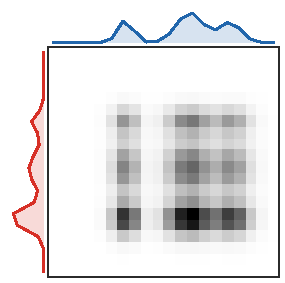
\includegraphics[width=.22\linewidth]{figures/kantorovich-coupling-matrix-marginals/product-20.pdf} &
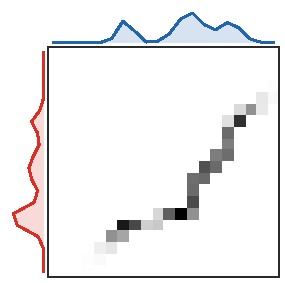
\includegraphics[width=.22\linewidth]{figures/kantorovich-coupling-matrix-marginals/optimal-20.pdf} &

\includegraphics[width=.22\linewidth]{figures/kantorovich-coupling-matrix-marginals/product-200.pdf} &

\includegraphics[width=.22\linewidth]{figures/kantorovich-coupling-matrix-marginals/optimal-200.pdf}
\end{tabular}
\caption{Coupling matrices with their prescribed marginals. The central grayscale image displays $P_{ij}$; the red curve on the left is the source marginal $\a$, the blue curve on top is the target marginal $\b$, and the thin red curve inside the matrix is the barycentric projection $i\mapsto\sum_j P_{ij}j/a_i$. The independent product plan is diffuse, whereas the one-dimensional optimal plan concentrates near the monotone quantile correspondence. The dense discretization is the same construction with 200 bins.}
\label{fig:kantorovich-coupling-matrix-marginals}
\end{figure}

\begin{figure}[H]
\centering
\begin{tabular}{@{}cccc@{}}
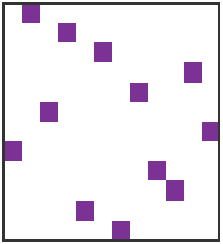
\includegraphics[width=.18\linewidth]{figures/kantorovich-permutation-versus-splitting/permutation-matrix.pdf} &

\includegraphics[width=.23\linewidth]{figures/kantorovich-permutation-versus-splitting/permutation-transport.pdf} &

\includegraphics[width=.16\linewidth]{figures/kantorovich-permutation-versus-splitting/splitting-matrix.pdf} &
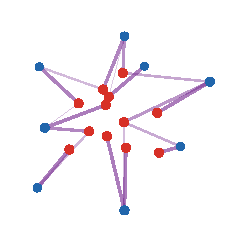
\includegraphics[width=.23\linewidth]{figures/kantorovich-permutation-versus-splitting/splitting-transport.pdf} \\[-.1em]
\small permutation matrix $\P_\sigma$ &
\small assignment segments &
\small splitting matrix $\P$ &
\small splitting segments
\end{tabular}
\caption{From permutation matrices to splitting couplings. When the two empirical measures have the same number of atoms and uniform weights, an optimal plan can be a permutation matrix. Once target masses are nonuniform, the admissible set $\CouplingsD(\a,\b)$ also contains plans in which one source sends mass to several targets and several sources merge into the same target.}
\label{fig:kantorovich-permutation-versus-splitting}
\end{figure}

\paragraph{Continuous couplings and plans.}
\label{sec-kantorovich-continuous}

The same relaxation applies to arbitrary probability measures. A transport plan is a joint probability measure with prescribed marginals.

\begin{defn}[Continuous couplings]\label{def-continuous-couplings}
	For $\al\in\Mm_+^1(\Xx)$ and $\be\in\Mm_+^1(\Yy)$, the set of couplings is
	\eql{\label{eq-coupling-generic}
		\Couplings(\al,\be)
		\eqdef
		\enscond{\pi\in\Mm_+^1(\Xx\times\Yy)}
		{(P_\Xx)_\sharp\pi=\al,\ (P_\Yy)_\sharp\pi=\be},
	}
	where $P_\Xx(x,y)=x$ and $P_\Yy(x,y)=y$.
\end{defn}

The Kantorovich optimal transport value is
\eql{\label{eq-mk-generic}
	\MK_\c(\al,\be)
	\eqdef
	\inf_{\pi\in\Couplings(\al,\be)}
	\int_{\Xx\times\Yy} c(x,y)\d\pi(x,y).
}
The product measure $\al\otimes\be$ is always feasible, so the relaxation is never empty, unlike the Monge constraint.

\begin{defn}[$c$-cyclical monotonicity]\label{def:ccm}
	A set $\Gamma\subset\Xx\times\Yy$ is $c$-cyclically monotone if, for every finite family $(x_i,y_i)_{i=1}^k\subset\Gamma$ and every permutation $\sigma$ of $\{1,\ldots,k\}$,
	\[
		\sum_{i=1}^k c(x_i,y_i)
		\leq
		\sum_{i=1}^k c(x_i,y_{\sigma(i)}).
	\]
\end{defn}

%
Additionally, whereas the Monge formulation is intrinsically asymmetric, Kantorovich's relaxed formulation is always symmetric, in the sense that a coupling $\P$ is in $\CouplingsD(\a,\b)$ if and only if $\transp{\P}$ is in $\CouplingsD(\b,\a)$.

Kantorovich, aiming for economic planning, made a strong simplifying assumption: the cost of transportation should be linear in the amount of transported mass.
%
Under this assumption, denoting $\C_{i,j}$ the cost of moving a unit amount of mass from $x_i$ to $y_j$, Kantorovich's optimal transport problem now reads
\eql{\label{eq-kanto-discr}
	\MKD_{\C}(\a,\b) \eqdef
	\umin{\P \in \CouplingsD(\a,\b)}
		\dotp{\C}{\P} \eqdef \sum_{i,j} \C_{i,j} \P_{i,j}.
}
This is a linear program, and as is usually the case with such programs, its solutions are not necessarily unique.

\begin{figure}[H]
\centering
\begin{tabular}{@{}ccc@{}}
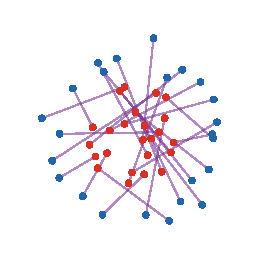
\includegraphics[width=.28\linewidth]{figures/kantorovich-coupling-polylines/graph.pdf} &
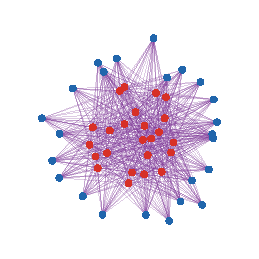
\includegraphics[width=.28\linewidth]{figures/kantorovich-coupling-polylines/product.pdf} &
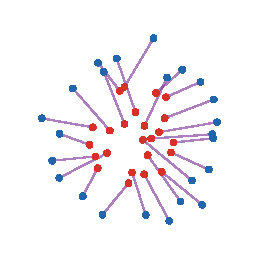
\includegraphics[width=.28\linewidth]{figures/kantorovich-coupling-polylines/optimal.pdf} \\[-.1em]
\small deterministic graph & \small product plan $\a\otimes\b$ & \small optimal plan
\end{tabular}
\caption{Discrete couplings represented as transport polylines on the canonical point clouds used in the matching section. The deterministic graph is a feasible Monge-type plan, the product plan spreads every source mass over all targets, and the optimal Kantorovich plan minimizes the quadratic transport cost. Line width and opacity encode the transported mass.}
\label{fig:kantorovich-coupling-polylines}
\end{figure}

\paragraph{Sparse feasible plans.}

Although the product plan $\a\otimes\b$ is always feasible, it is dense and therefore a poor initialization for algorithms that exploit sparsity. The transportation polytope always contains sparse feasible points, and linear costs always admit sparse optimizers.

\begin{prop}[Sparse optimal plans]\label{prop-sparse-optimal-plans}
	Assume $\a_i>0$, $\b_j>0$ and $\sum_i a_i=\sum_j b_j=1$. The linear program~\eqref{eq-kanto-discr} admits an optimal coupling with at most $n+m-1$ nonzero entries.
\end{prop}

\begin{proof}
	The transportation polytope is compact, so a linear objective attains its minimum at an extreme point. We show that any extreme point has at most $n+m-1$ positive entries. Let $E=\{(i,j):P_{ij}>0\}$ be the support graph on the bipartite vertex set $\{1,\ldots,n\}\cup\{1,\ldots,m\}$. If this graph contains a cycle, orient the cycle and put alternating signs $+1,-1$ on its edges, obtaining a nonzero matrix $H$ supported on $E$ with zero row and column sums. For sufficiently small $t>0$, both $P+tH$ and $P-tH$ are nonnegative couplings, and $P$ is their midpoint, contradicting extremality. Thus the support graph is a forest. Since a forest on $n+m$ vertices has at most $n+m-1$ edges, the claim follows.
\end{proof}

\begin{prop}[North-west corner feasible plan]\label{prop-northwest-corner}
	For any $\a\in\simplex_n$ and $\b\in\simplex_m$, the following algorithm returns a coupling in $\CouplingsD(\a,\b)$ with at most $n+m-1$ nonzero entries. Initialize residuals $r_i=a_i$, $s_j=b_j$ and indices $i=j=1$. While $i\leq n$ and $j\leq m$, set
	\[
		P_{ij}=\min(r_i,s_j),
	\]
	replace $r_i\leftarrow r_i-P_{ij}$ and $s_j\leftarrow s_j-P_{ij}$, then increase every index whose residual is zero.
\end{prop}

\begin{proof}
	At each step the algorithm assigns the largest possible mass to the current cell without violating either the current row or current column constraint. The residuals remain nonnegative, and at least one of them becomes zero, so at least one index advances. Hence the procedure terminates after at most $n+m-1$ assignments unless a final simultaneous row/column exhaustion ends the algorithm earlier. Each row $i$ receives exactly its initial mass $a_i$ before the index moves past it, and each column $j$ receives exactly $b_j$ before the column index moves past it. Therefore the output has row sums $\a$, column sums $\b$, nonnegative entries, and at most one new nonzero per step. In one dimension this is the discrete quantile sweep, hence the discrete analogue of the Knothe--Rosenblatt axis-wise construction of Proposition~\ref{prop-knothe-rosenblatt}.
\end{proof}

\begin{prop}[One-dimensional weighted sweep]\label{prop-1d-weighted-sweep}
	Let $x_1\leq\cdots\leq x_n$ and $y_1\leq\cdots\leq y_m$ be points on the line, and let $c(x,y)=h(x-y)$ with $h$ convex. The north-west corner plan between the sorted weighted atoms is optimal for~\eqref{eq-kanto-discr}. Consequently, for unsorted one-dimensional inputs, an optimal plan is obtained in $O(n\log n+m\log m)$ time by sorting and then sweeping the masses once from left to right.
\end{prop}

\begin{proof}
	The north-west plan is monotone: if $i<i'$ and $j>j'$, it cannot put positive mass on both $(i,j)$ and $(i',j')$, because the sweep exhausts rows and columns in increasing order. Conversely, any feasible plan with a crossing pair of positive entries can be improved by moving a small mass $\eta$ from $(i,j)$ and $(i',j')$ to $(i,j')$ and $(i',j)$. The two marginals are unchanged, and convexity of $h$ gives
	\[
		h(x_i-y_j)+h(x_{i'}-y_{j'})
		\geq
		h(x_i-y_{j'})+h(x_{i'}-y_j)
	\]
	for $i<i'$ and $j'<j$, with strict inequality for strictly convex $h$ and distinct points. Repeating this uncrossing procedure until no crossing remains yields a monotone optimal plan. There is only one monotone feasible plan with the prescribed sorted marginals, namely the sweep plan: it pairs the leftmost remaining source mass with the leftmost remaining target mass at every step. Sorting costs $O(n\log n+m\log m)$ and the sweep uses at most $n+m-1$ assignments.
\end{proof}


\paragraph{Optimal matching to optimal transport.}

Let the marginals be uniform on $n$ points: $\alpha=\tfrac1n\sum_{i=1}^n\delta_{x_i}$, $\beta =\tfrac1n\sum_{i=1}^n\delta_{y_i}$.
In this case, there exist solutions to the Kantorovich problem that are permutations.
Such a permutation defines, by optimality, a coupling with support $\Gamma := (x_i,y_{\sigma(i)})_i$ that is $c$-cyclically monotone.
The following theorem says this is true for any optimal coupling, not only in the case of a finite set of points.

\begin{thm}[Rockafellar]\label{thm:opt_ccm}
For any optimal plan $\pi$ solving Kantorovich's problem,
$\supp(\pi)$ is $c$-cyclically monotone.
\end{thm}
\begin{proof}
	We prove the contrapositive. Suppose that $\supp(\pi)$ is not $c$-cyclically monotone. Then there exist points $(x_i,y_i)_{i=1}^k$ in the support and a permutation $\sigma$ such that
	\[
		\sum_i c(x_i,y_i) >
		\sum_i c(x_i,y_{\sigma(i)}).
	\]
	By continuity of $c$, this strict inequality persists on small neighborhoods $U_i\times V_i$ of the points $(x_i,y_i)$, chosen disjoint enough so that each has positive $\pi$-mass. Let $\eta>0$ be smaller than all these masses. Removing mass $\eta$ from each $U_i\times V_i$ and re-inserting the same mass from $U_i$ to $V_{\sigma(i)}$ preserves both marginals, because the operation only permutes target neighborhoods among the same source neighborhoods. The cost strictly decreases by the displayed gap up to the continuity error. This contradicts optimality of $\pi$.
\end{proof}

\paragraph{Interpolation induced by a plan.}

A transport plan also defines an interpolation between measures by moving every active pair $(x_i,y_j)$ along the segment $(1-t)x_i+t y_j$ with mass $\P_{ij}$. When the plan is not induced by a map, one source atom can split into several moving atoms.

\begin{figure}[H]
\centering
\begin{tabular}{@{}ccccc@{}}
\small $t=0$ & \small $t=1/4$ & \small $t=1/2$ & \small $t=3/4$ & \small $t=1$ \\[-.15em]

\includegraphics[width=.17\linewidth]{figures/kantorovich-plan-interpolation/time-000.pdf} &
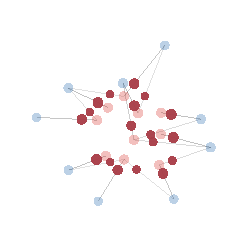
\includegraphics[width=.17\linewidth]{figures/kantorovich-plan-interpolation/time-025.pdf} &
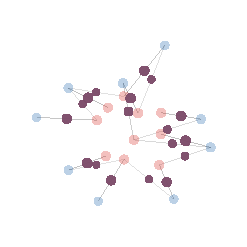
\includegraphics[width=.17\linewidth]{figures/kantorovich-plan-interpolation/time-050.pdf} &
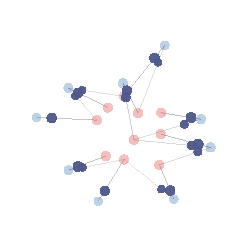
\includegraphics[width=.17\linewidth]{figures/kantorovich-plan-interpolation/time-075.pdf} &
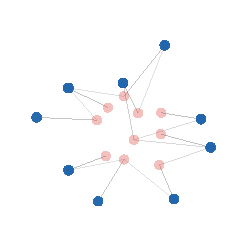
\includegraphics[width=.17\linewidth]{figures/kantorovich-plan-interpolation/time-100.pdf}
\end{tabular}
\caption{McCann interpolation induced by a non-deterministic transport plan. In every panel, the red and blue endpoint measures are shown with low opacity, thin gray segments display the support $P_{ij}>\mathrm{tol}$ of the coupling, and the moving atoms are colored from red to blue along the interpolation.}
\label{fig:kantorovich-plan-interpolation}
\end{figure}


\paragraph{Monotonicity.}

Assume the plan is induced by a measurable map
$T:\X\to \Y$, i.e.\ $\pi=(\Id,T)_\#\alpha$.
For any $k$ points $x_1,\dots,x_k$ in the domain, cyclical
monotonicity reads
\[
  \sum_{i=1}^k c\bigl(x_i,T(x_i)\bigr)
  \;\le\;
  \sum_{i=1}^k c\bigl(x_i,T(x_{i+1})\bigr),\qquad x_{k+1}=x_1.
\]
For $c(x,y)=\tfrac12|x-y|^2$, taking $k=2$, shows that for any $x,y$,
\[
  \langle T(x)-T(y),\,x-y\rangle\;\ge\;0,
\]
so $T$ is a monotone vector field.
Brenier's theorem adds that, when $\alpha$ is absolutely continuous,
$T=\nabla\varphi$ for a convex potential $\varphi$.
(The converse fails in dimension $d\ge2$: a small rotation is monotone
yet not a gradient.)

\paragraph{One dimension.}

In one space dimension, with cost $c(x,y)=|x-y|^p$ for any $p\ge1$, the
two-point inequality becomes
\[
  |x-T(x)|^p+|y-T(y)|^p
  \;\le\;
  |x-T(y)|^p+|y-T(x)|^p,
\]
which is equivalent to $T(x)\le T(y)$ whenever $x<y$. Thus $T$ must be
non-decreasing, recovering the classical monotone rearrangement.

%%%%%%%%%%%%%%%%%%%%%%%%%%%%%%%%%%%%%%%%%%%%%%%%%%%%%%%%%%%%%%%%%%%%%%%%%%%
\subsection{Metric Properties: Wasserstein Distances}


The final part of the section proves that OT costs are genuine distances when the ground cost comes from a metric. It also compares Wasserstein convergence with total variation and explains why OT is weak enough to move Dirac masses continuously.

%%%%
\paragraph{OT defines a distance.}


An important feature of OT is that it defines a distance between histograms and probability measures as soon as the cost matrix satisfies certain suitable properties. Indeed, OT can be understood as a canonical way to lift a ground distance between points to a distance between histograms or measures.
%
The proof of this result relies on a ``gluing lemma'', which we first prove in the discrete case.

\begin{lem}[Discrete gluing lemma]\label{lem-gluing-discr}
	Given $(\a,\b,\VectMode{c}) \in \simplex_n \times \simplex_p \times \simplex_m$,
	let $\P \in \CouplingsD(\a,\b)$ and $\Q \in \CouplingsD(\b,\VectMode{c})$. Then there exists a 3-D tensor coupling $\S \in \RR_+^{n \times p \times m}$
	such that the 2-D marginals satisfy
	\eq{
		\sum_{k} \S_{i,j,k} = \P_{i,j}
		\qandq
		\sum_{i} \S_{i,j,k} = \Q_{j,k}.
	}
	Note that this implies that the three 1-D marginals of $\S$ are $(\a,\b,\VectMode{c})$.
\end{lem}
\begin{proof}
	One verifies that
	\eql{\label{eq-glued-discr}
		\S_{i,j,k} = \choice{
			\frac{\P_{i,j} \Q_{j,k}}{\b_j}  \qifq \b_j \neq 0 \\
			0 \text{ otherwise}
		}
	}
	is acceptable. Indeed, if $\b_j \neq 0$
	\eq{
		\sum_{k} \S_{i,j,k} = \sum_{k} \frac{\P_{i,j} \Q_{j,k}}{\b_j}
		= \frac{\P_{i,j}}{\b_j} ( \Q \ones_m )_j = \frac{\P_{i,j}}{\b_j}  \b_j.
	}
	If $\b_j = 0$, then necessarily $\P_{i,j}=0$ and $\sum_{k} \S_{i,j,k} = 0 = \P_{i,j}$.
\end{proof}

\begin{figure}[H]
\centering
\begin{tabular}{@{}cccc@{}}
\small $P\in\CouplingsD(\a,\b)$ & \small $Q\in\CouplingsD(\b,\VectMode{c})$ & \small glued $R$ & \small direct OT \\[-.15em]

\includegraphics[width=.22\linewidth]{figures/kantorovich-discrete-gluing-lemma/ab-plan.pdf} &
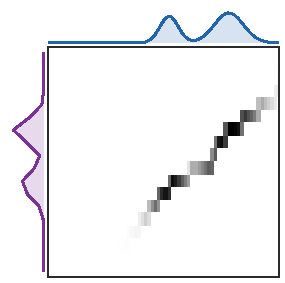
\includegraphics[width=.22\linewidth]{figures/kantorovich-discrete-gluing-lemma/bc-plan.pdf} &
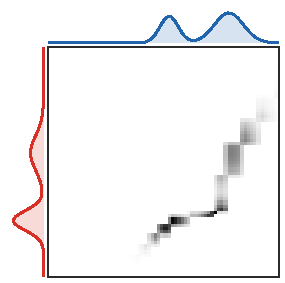
\includegraphics[width=.22\linewidth]{figures/kantorovich-discrete-gluing-lemma/glued-ac-plan.pdf} &

\includegraphics[width=.22\linewidth]{figures/kantorovich-discrete-gluing-lemma/direct-ac-plan.pdf}
\end{tabular}
\caption{Discrete gluing lemma in matrix form. The first two panels are optimal one-dimensional couplings through an intermediate marginal $\b$. The third panel shows the induced marginal $R=P\diag(1/\b)Q$ between $\a$ and $\VectMode{c}$; it is feasible and is the coupling used in the triangle-inequality proof. Because the intermediate marginal is represented on a coarser grid, the glued coupling is more mediated than the direct optimal coupling shown on the right.}
\label{fig:kantorovich-discrete-gluing-lemma}
\end{figure}

% We first consider the case where, using a term first introduce by~\cite{RubTomGui00}, the ``ground metric'' matrix $\C$ is fixed, representing substitution costs between bins, and shared across several histograms we would like to compare. The following proposition states that OT provides a meaningful distance between histograms supported on these bins.

\begin{prop}[Discrete Wasserstein distance]\label{prop-metric-histo}
We suppose $n=m$, and that for some $p \geq 1$, $\C=\distD^p=(\distD_{i,j}^p)_{i,j} \in \RR^{n \times n}$ where $\distD \in \RR_+^{n \times n}$ is a distance on $\range{n}$, \emph{i.e.}
\begin{enumerate}% [label=(\roman*)]
	\item $\distD \in \RR_+^{n \times n}$ is symmetric;
	\item $\distD_{i,j}=0$ if and only if $i=j$;
	\item $\foralls (i,j,k) \in \range{n}^3, \distD_{i,k} \leq \distD_{i,j}+\distD_{j,k}$.
\end{enumerate}
Then
\eql{\label{eq-wass-p-disc}
	\WassD_p(\a,\b) \eqdef \MKD_{\distD^p}(\a,\b)^{1/p}
}
(note that $\WassD_p$ depends on $\distD$) defines the $p$-Wasserstein distance on $\Si_n$, \emph{i.e.} $\WassD_p$ is symmetric, positive, $\WassD_p(\a,\b)=0$ if and only if $\a = \b$, and it satisfies the triangle inequality
\eq{
	\foralls \a,\b,\VectMode{c} \in \Si_n, \quad \WassD_p(\a,\VectMode{c}) \leq \WassD_p(\a,\b) + \WassD_p(\b,\VectMode{c}).
}
\end{prop}

\begin{proof}
For symmetry, since $\distD^p$ is symmetric, we use the fact that if $\P \in \CouplingsD(\a,\b)$ is optimal for $\WassD_p(\a,\b)$, then $\P^\top \in \CouplingsD(\b,\a)$ is optimal for $\WassD_p(\b,\a)$. For definiteness, since $\C = \distD^p$ has a null diagonal, $\WassD_p(\a,\b)=0$ is achieved by the diagonal coupling $\P^\star=\diag(\a)=\diag(\b)$ when $\a=\b$; by positivity of all off-diagonal elements of $\distD^p$, $\WassD_p(\a,\b)>0$ whenever $\a\ne \b$ because any admissible coupling then has a nonzero element outside the diagonal.

To prove the triangle inequality of Wasserstein distances for arbitrary measures, we consider $\a,\b,\VectMode{c} \in\simplex_n$, and let $\P$ and $\Q$ be two optimal solutions of the transport problems between $\a$ and $\b$, and $\b$ and $\VectMode{c}$ respectively.
%
We use the gluing Lemma~\ref{lem-gluing-discr} which defines $\S \in \RR_+^{n^3}$ with marginals $\sum_{k}\S_{\cdot,\cdot,k}=\P$ and $\sum_i \S_{i,\cdot,\cdot}=\Q$. We define $\R=\sum_{j}\S_{\cdot,j,\cdot}$, which is an element of $\CouplingsD(\a,\VectMode{c})$.
\[
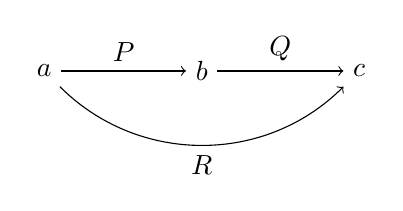
\begin{tikzpicture}
  \node (a) at (0,0) {$a$};
  \node (b) at (2,0) {$b$};
  \node (c) at (4,0) {$c$};

  \draw[->] (a) -- (b) node[midway, above] {$P$};
  \draw[->] (b) -- (c) node[midway, above] {$Q$};
  \draw[->, bend right=45] (a) to node[midway, below] {$R$} (c);
\end{tikzpicture}
\]
Note that if one assumes $\b>0$ then $\R = \P \diag(1/\b) \Q$.
%

The triangle inequality follows from
$$\begin{aligned}
\WassD_p(\a,\VectMode{c})&=\Big(\min_{\tilde\R\in \CouplingsD(\a,\VectMode{c})}\dotp{\tilde\R}{\distD^p}\Big)^{1/p} \leq \dotp{\R}{\distD^p}^{1/p}\\
&= \Big(\sum_{i,k}  \distD^p_{ik}\sum_{j} \S_{i,j,k} \Big)^{1/p}
 \leq \Big(\sum_{i,j,k} \left(\distD_{ij}+\distD_{j,k}\Big)^p  \S_{i,j,k} \right)^{1/p} \\
& \leq \Big(\sum_{i,j,k} \distD^p_{ij} \S_{i,j,k} \Big)^{1/p} + \Big(\sum_{i,j,k}\distD^p_{j,k} \S_{i,j,k} \Big)^{1/p} \\
&= \Big(\sum_{i,j} \distD^p_{i,j}  \sum_k \S_{i,j,k} \Big)^{1/p} + \Big(\sum_{j,k} \distD^p_{j,k}  \sum_i \S_{i,j,k} \Big)^{1/p}\\
&= \Big(\sum_{i,j} \distD^p_{i,j}\P_{i,j}\Big)^{1/p} + \Big(\sum_{j,k} \distD^p_{j,k} \Q_{j,k}\Big)^{1/p}
= \WassD_p(\a,\b) +\WassD_p(\b,\VectMode{c}).
\end{aligned}
$$
%
The first inequality follows from the feasibility of $\R$, the second is the usual triangle inequality for elements in $\distD$, and the third comes from Minkowski's inequality.
\end{proof}

\paragraph{Continuous gluing.}

Proposition~\ref{prop-metric-histo} generalizes from histogram to arbitrary measures that need not be discrete. For this, one needs the following general gluing lemma.

\begin{lem}[Gluing lemma]\label{lem-gluing-general}
	Let $(\al,\be,\ga) \in \Mm_+^1(\Xx) \times \Mm_+^1(\Yy) \times \Mm_+^1(\Zz)$
	where $(\Xx,\Yy,\Zz)$ are Polish spaces, i.e. separable topological spaces that can be metrized by complete distances.
	%
	Given $\pi \in \Couplings(\al,\be)$ and $\xi \in \Couplings(\be,\ga)$, then there exists a tensor coupling measure
	$\sigma \in \Mm_+(\Xx \times \Yy \times \Zz)$ such that
	\eq{
		(P_{\Xx,\Yy})_\sharp \sigma = \pi
		\qandq
		(P_{\Yy,\Zz})_\sharp \sigma = \xi
	}
	where we denoted the projector $P_{\Xx,\Yy}(x,y,z)=(x,y)$ and $P_{\Yy,\Zz}(x,y,z)=(y,z)$.
\end{lem}
\begin{proof}
	The proof of this fundamental result is involved since it requires using the disintegration of measure (which corresponds to conditional probabilities).
	%
	The disintegration of measures is applicable because the spaces are Polish.
	%
	We disintegrate $\pi$ and $\xi$ against $\be$ to obtain two families $(\pi_y)_{y \in \Yy}$ and $(\xi_y)_{y \in \Yy}$ of probability distributions on $\Xx$ and $\Zz$. These families are defined by the fact that
	\eq{
		\foralls h \in \Cc(\Xx \times \Yy), \quad
		\int_\Yy \Big( \int_\Xx h(x,y) \d \pi_y(x) \Big) \d \be(y) = \int h(x,y) \d\pi(x,y).
	}
	and similarly for $\xi$.
	%
	When $\be=\sum_j \b_j \de_{y_j}$ and $\pi=\sum_{i,j} \P_{i,j} \de_{(x_i,y_j)}$, then this conditional distribution is defined on the support of $\be$ as
	$\pi_{y_j} = \sum_i \frac{\P_{i,j}}{\b_j} \de_{x_i}$ (and similarly for $\xi$).
	%
		The glued measure is then defined by the conditional-product formula
	\eq{
		\foralls g \in \Cc(\Xx \times \Yy \times \Zz), \quad
		\int g(x,y,z) \d\sigma(x,y,z) = \int g(x,y,z) \d \pi_y(x) \d \xi_y(z) \d \be(y).
	}
	For discrete measures, this matches the definition~\eqref{eq-glued-discr}, since $\sigma=\sum_{i,j,k} \S_{i,j,k} \de_{x_i,y_j,z_k}$ where
	\eq{
		\S_{i,j,k} = \frac{\P_{i,j}}{\b_j} \frac{\Q_{j,k}}{\b_j} \b_j.
	}
\end{proof}

Using this gluing lemma, we can now construct the Wasserstein distance in the general setting of arbitrary distributions on a Polish space.

\begin{prop}[Wasserstein distance on measures]\label{prop-metric-measure}
We assume $\X=\Y$, and that for some $p \geq 1$, $\c(x,y)=\dist(x,y)^p$ where $\dist$ is a distance on $\X$, \emph{i.e.} \\
	\hbox{}\qquad (i) $\dist(x,y) = \dist(y,x) \geq 0$;  \\
	\hbox{}\qquad (ii)  $\dist(x,y)=0$ if and only if $x=y$;  \\
	\hbox{}\qquad (iii)  $\foralls (x,y,z) \in \X^3, \dist(x,z) \leq \dist(x,y)+\dist(y,z)$. \\
Then
\eql{\label{eq-defn-wass-dist}
	\Wass_p(\al,\be) \eqdef \MK_{\dist^p}(\al,\be)^{1/p}
}
(note that $\Wass_p$ depends on $\dist$) defines the $p$-Wasserstein distance on $\X$, \emph{i.e.} $\Wass_p$ is symmetric, positive, $\Wass_p(\al,\be)=0$ if and only if $\al = \be$, and it satisfies the triangle inequality
\eq{
	\foralls (\al,\be,\ga) \in  \Mm_+^1(\X)^3, \quad \Wass_p(\al,\ga) \leq \Wass_p(\al,\be) + \Wass_p(\be,\ga).
}
\end{prop}

\begin{proof}
	The symmetry follows from the fact that since $\dist$ is symmetric, if $\pi(x,y)$ is optimal for $\MK_{\dist^p}(\al,\be)$, then
	$\pi(y,x) \in \Couplings(\be,\al)$ is optimal for $\MK_{\dist^p}(\be,\al)$.
	%
	If $\MK_{\dist^p}(\al,\be)=0$, then necessarily an optimal coupling $\pi$ is supported on the diagonal $\De \eqdef \{(x,x)\}_x \subset \Xx^2$.
	%
	We denote $\la(x)$ the corresponding measure on the diagonal, i.e. such that $\int h(x,y) \d\pi(x,y) = \int h(x,x) \d \la(x)$.
	%
	Then since $\pi \in \Couplings(\al,\be)$ necessarily $\la=\al$ and $\la=\be$ so that $\al=\be$.

	For the triangle inequality, we consider optimal couplings $\pi \in \Couplings(\al,\be)$ and $\xi \in \Couplings(\be,\ga)$
	and we glue them according to the Lemma~\ref{lem-gluing-general}.
	%
		We define the composition of the two couplings $(\pi,\xi)$ as $\rho \eqdef (P_{\Xx,\Zz})_\sharp \si$.
	%
	Note that if $\pi$ and $\xi$ are couplings induced by two Monge maps $T_\Xx(x)$ and $T_\Yy(y)$, then $\rho$ is itself induced by the Monge map $T_\Yy \circ T_\Xx$, so that this notion of composition of coupling generalizes the composition of maps.
	%
	The triangular inequality follows from
	$$\begin{aligned}
		\Wass_p(\al,\ga) & \leq \Big( \int_{\Xx \times \Zz} \dist(x,z)^p \d\rho(x,z)\Big)^{1/p}
		= \Big( \int_{\Xx \times \Yy \times \Zz} \dist(x,z)^p \d\si(x,y,z)\Big)^{1/p}		\\
		 &\leq \Big( \int_{\Xx \times \Yy \times \Zz} (\dist(x,y)+\dist(y,z))^p \d\si(x,y,z)\Big)^{1/p} \\
		 &\leq \Big( \int_{\Xx \times \Yy \times \Zz} \dist(x,y)^p \d\si(x,y,z)\Big)^{1/p}
		    +  \Big( \int_{\Xx \times \Yy \times \Zz} \dist(y,z)^p \d\si(x,y,z)\Big)^{1/p} \\
	  &= \Big( \int_{\Xx \times \Yy} \dist(x,y)^p \d\pi(x,y)\Big)^{1/p}
		    +  \Big( \int_{\Yy \times \Zz} \dist(y,z)^p \d\xi(y,z)\Big)^{1/p}
		    = \Wass_p(\al,\be)  + \Wass_p(\be,\ga) .
	\end{aligned}$$
\end{proof}

\paragraph{Comparison with Monge.}

	This distance $\Wass_p$ defined through the Kantorovich problem~\eqref{eq-defn-wass-dist} should be contrasted with the directed distance $\tilde\Wass$ obtained using Monge's problem~\eqref{eq-monge-distance}. The Kantorovich feasible set is never empty, since it contains the product coupling, although the $p$-cost may still be infinite without moment assumptions on non-compact spaces. By contrast, Monge's constraint set $\enscond{T}{T_\sharp \al=\be}$ can be empty. When an optimal Monge map exists, Kantorovich gives the same value by choosing the graph coupling $(\Id,T)_\sharp\alpha$; in this sense the Kantorovich problem is the convex relaxation of Monge's problem, with much better stability properties.


%%%%
\subsection{Metric Properties: Topology and Applications}

This subsection shifts from metric axioms to topology and uses. Wasserstein distances metrize weak convergence under moment control, sit between weak and strong topologies, and provide quantitative estimates in probability and robust optimization.

\paragraph{Convergence in law topology.}

On a bounded metric space, all $\Wass_p$ distances define the same topology, although they are not equivalent as distances.

\begin{prop}[Equivalence of Wasserstein distances on compact spaces]\label{prop-comp-wass-p}
	One has for $p \leq q$
	\eq{
		\Wass_p( \al,\be ) \leq \Wass_q(\al,\be) \leq \text{\upshape diam}(\Xx)^{\frac{q-p}{q}} \Wass_p(\al,\be)^{\frac{p}{q}}
	}
	where $\text{\upshape diam}(\Xx) \eqdef \usup{x,y} d(x,y)$.
\end{prop}
\begin{proof}
		The left inequality follows from Jensen inequality, $\phi(\int c(x,y) \d\pi(x,y)) \leq \int \phi(c(x,y)) \d\pi(x,y)$, applied to any probability distribution $\pi$ and to the convex function $\phi(r)=r^{q/p}$ with $c(x,y)=d(x,y)^p$, so that one gets
		\eq{
			\pa{\int d(x,y)^{p} \d\pi(x,y)}^{\frac{q}{p}} \leq \int d(x,y)^{q} \d\pi(x,y).
		}
		The right inequality follows from
		\eq{
			d(x,y)^q \leq \text{diam}(\Xx)^{q-p} d(x,y)^p.
		}
	\end{proof}

The Wasserstein distance $\Wass_p$ is a weak distance: it compares singular distributions, such as discrete measures, and quantifies spatial shifts between supports. Its topology is studied in detail in~\cite{Villani09,SantambrogioBook,gigli2011user}, while empirical rates are quantified in~\cite{dudley1969speed,fournier2015rate,weed2017sharp,boissard2015distribution,bolley2007quantitative}.

\begin{defn}[Weak$^*$ topology]\label{dfn-weak-conv}
	$(\al_k)_k$ converges weakly$^*$ to $\al$ in $\Mm_+^1(\Xx)$ (denoted $\al_k \rightharpoonup \al$) if and only if for any bounded continuous function $f \in \Cc_b(\Xx)$, $\int_\Xx f \d\al_k \rightarrow \int_\Xx f \d\al$. On compact spaces, $\Cc_b(\Xx)=\Cc(\Xx)$, which is why the boundedness is often left implicit there.
\end{defn}

\begin{rem}[A Riemann-sum weak limit]\label{rem-riemann-weak-limit}
	On $\Xx=\RR$, the empirical measures on a regular grid satisfy
	\[
		\frac{1}{n} \sum_{k=1}^n \de_{k/n} \rightharpoonup \Uu_{[0,1]}.
	\]
	Indeed, for every continuous bounded function $f$,
	\[
		\frac{1}{n} \sum_{k=1}^n f(k/n) \longrightarrow \int_0^1 f(x) \d x,
	\]
	which is precisely the convergence of Riemann sums. This convergence is weak but not strong: for every $n$, the discrete measure and the uniform density are mutually singular, hence their total variation distance is equal to $2$.
\end{rem}

\begin{rem}[Weak convergence for discrete measures]\label{rem-weak-conv-disc}
	In the special case of a single Dirac, $\de_{x^{(n)}} \rightharpoonup \de_x$ is equivalent to $\int f \d\de_{x^{(n)}} = f(x^{(n)}) \rightarrow \int f \d\de_{x} = f(x)$ for any continuous $f$. This in turn is equivalent to $x^{(n)} \rightarrow x$.
	For a fixed number of atoms, if $\al_n=\sum_{i=1}^N a_i^{(n)}\de_{x_i^{(n)}}$ and, after extracting a subsequence and relabeling, $a_i^{(n)}\to a_i$ and $x_i^{(n)}\to x_i$, then $\al_n$ converges weakly to $\sum_i a_i\de_{x_i}$, with atoms at identical limits merged. Without a uniform bound on the number of atoms, weak limits of discrete measures can be non-discrete; empirical measures are the standard example.
\end{rem}

In terms of random vectors, if $X_n \sim \al_n$ and $X \sim \al$ (not necessarily defined on the same probability space), weak convergence corresponds to convergence in law of $X_n$ toward $X$.

\begin{rem}[Central limit theorem]\label{rem-clt}
		The central limit theorem states that if $(X_1,\ldots,X_n)$ are i.i.d. random vectors with finite second moments, $\EE(X_i)=0$, and $\EE(X_i X_i^\top)=\Id$, then the rescaled average $Z_n \eqdef \frac{1}{\sqrt{n}} \sum_{i=1}^n X_i$ converges in law toward a Gaussian $\Gaussian(0,\Id)$. This means that the measure $\al_n$ representing the law of $Z_n$ converges weakly toward the measure $\al$ of the centered normalized Gaussian.
\end{rem}

\begin{defn}[Strong topology]
The simplest distance on Radon measures is the total variation norm, which is the dual norm of the $L^\infty$ norm on $\Cc(\Xx)$ and whose topology is often called the ``strong'' topology
\eq{
	\norm{\al-\be}_{\TV} \eqdef \usup{\norm{f}_\infty \leq 1} \int f \d(\al-\be)
	 = |\al-\be|(\Xx)
}
where $|\al-\be|(\Xx)$ is the mass of the absolute value of the difference measure. When $\al-\be=\rho \d x$ has a density, then $\norm{\al-\be}_{\TV}=\int |\rho(x)| \d x=\norm{\rho}_{L^1(\d x)}$ is the $L^1$ norm associated to $\d x$. When $\al-\be=\sum_i u_i \de_{z_i}$ is discrete, then $\norm{\al-\be}_{\TV}=\sum_i |u_i|=\norm{u}_{\ell^1}$ is the discrete $\ell^1$ norm.
\end{defn}

The following proposition shows that the TV norm can be seen as a Wasserstein distance, but for a ``degenerate'' 0/1 metric.

\begin{prop}[Total variation as Wasserstein for the discrete metric]\label{prop-rel-wass-tv}
	Denoting $d$ the 0/1 distance such that $d(x,x)=0$ and $d(x,y)=1$ if $x \neq y$, then
	\eq{
		\Wass_p(\al,\be)^p = \frac{1}{2}\norm{\al-\be}_{\TV}.
	}
\end{prop}
\begin{proof}
	For the sake of simplicity, we do the proof for discrete measures with weights $(\a,\b)$ and without loss of generality assume they have the same support $(x_i)_i$ and we denote $\D \eqdef (d(x_i,x_j))_{i,j}$ which is 0 on the diagonal and one outside.
	%
	Also since $d^p=d$ we consider $p=1$.
	We denote $\text{c}_i = \min(\a_i,\b_i)$.
		By conservation of mass, for every $\P \in \CouplingsD(\a,\b)$, $\P_{i,i} \leq \text{c}_i$, thus
		\eq{
			\dotp{\P}{\D} = \sum_{i \neq j} \P_{i,j}
			= 1 - \sum_i \P_{i,i}
			\geq 1-\sum_i \text{c}_i.
		}
	We need to show that this bound is tight, namely to construct $\hat P \in \CouplingsD(\a,\b)$ such that
	$\diag(\hat P)=\text{c}$. Let
	\eq{
		\bar\a \eqdef \a-\text{c} = (\a-\b)_+ \geq 0
		\qandq
		\bar\b \eqdef \b-\text{c} = (\b-\a)_+ \geq 0
	}
	If $\bar\a=\bar\b=0$, then $\a=\b$ and the diagonal coupling is optimal. Otherwise, one has
		\eq{
			\frac{ \bar\a \otimes \bar\b }{ \dotp{\bar\a}{\ones} } \in \CouplingsD(\bar\a,\bar\b)
		}
		and we remark that $\dotp{\bar\a}{\ones} = \dotp{\bar\b}{\ones} = 1-\dotp{\text{c}}{\ones}$.
		%
		Thus denoting
		\eq{
			\hat \P \eqdef \diag(\text{c}) + \frac{ \bar\a \otimes \bar\b }{ \dotp{\bar\a}{\ones} } \geq 0
		}
	satisfies
	\eq{
			\hat\P \ones = \text{c} + \bar\a = \a
			\qandq
			\hat\P^\top \ones = \text{c} + \bar\b = \b
		}
		so that $\hat P \in \CouplingsD(\a,\b)$  is a coupling so that $\diag(\hat P) = \diag(\text{c})$ since $\diag( \bar\a \otimes \bar\b )=0$. We thus conclude that
		\eq{
			\WassD_1(\a,\b) = \dotp{\D}{\hat \P}
			= \sum_{i,j} \frac{\bar\a_i\bar\b_j}{\dotp{\bar\a}{\ones}}
		= \sum_i \bar\a_i = \sum_i \bar\b_i
		= \frac{1}{2} \sum_i (\bar\a_i + \bar\b_i)
		= \frac{1}{2} \norm{\a-\b}_{\TV}.
	}
\end{proof}


As explained in Remark~\ref{rem-weak-conv-disc}, in the special case of Diracs, $\de_{x_n} \rightharpoonup \de_x$  is equivalent to $x_n \rightarrow x$. One can then contrast the strong topology with the Wasserstein distance if $x_n \neq x$,
\eq{
	\norm{\de_{x_n}-\de_x}_{\TV}=2
	\qandq
	\Wass_p(\de_{x_n},\de_x) = d(x_n,x).
}
This shows that for the strong topology, Diracs never converge, while they do converge for the Wasserstein distance. It is a powerful property of the Wasserstein distance: on compact spaces, it metrizes weak convergence.

\begin{prop}[Wasserstein metrizes weak convergence on compact spaces]\label{prop-wass-metrizes-weak-compact}
	If $\Xx$ is compact, $\al_k \rightharpoonup \al$ if and only if $\Wass_p(\al_k,\al) \rightarrow 0$.
\end{prop}
\begin{proof}
	For $p=1$, this is the Kantorovich--Rubinstein metrization theorem: by duality, $\Wass_1$ is the supremum over $1$-Lipschitz test functions, and on a compact metric space this class is compact modulo constants by Arzel\`a--Ascoli. Thus convergence in $\Wass_1$ is equivalent to weak convergence. Proposition~\ref{prop-comp-wass-p} then shows that all Wasserstein distances $\Wass_p$ induce the same convergent sequences on compact spaces. Hence weak convergence is equivalent to convergence in $\Wass_p$ for every $p\geq1$.
\end{proof}

On non-compact spaces, one needs also to impose convergence of the $p$-th moments. More precisely, on a Polish metric space, $\Wass_p(\alpha_k,\alpha)\to0$ if and only if $\alpha_k\rightharpoonup\alpha$ and, for some reference point $x_0$,
\[
	\int d(x,x_0)^p\d\alpha_k(x)\longrightarrow
	\int d(x,x_0)^p\d\alpha(x).
\]
%
Note that there exist alternative distances which also metricize weak convergence. The simplest ones are Hilbertian kernel norms, which are detailed in Section~\ref{sec-dual-norms}.

On a discrete space, the strong and weak topologies coincide, and the following proposition relates the TV and Wasserstein distances.

\begin{prop}[Comparison with total variation on discrete spaces]
	One has
	\eq{
		\frac{d_{\min}}{2}\norm{\al-\be}_{\TV} \leq \Wass_1(\al,\be) \leq \frac{d_{\max}}{2}  \norm{\al-\be}_{\TV}
		\qwhereq
		\choice{
			d_{\min} \eqdef \uinf{x \neq y} d(x,y) \\
			d_{\max} \eqdef \usup{x,y} d(x,y)
		}
	}
\end{prop}

\begin{proof}
	We denote $d_0(x,y)$ the distance such that $d_0(x,x)=0$ and $d_0(x,y)=1$ for $x \neq y$. One has
	\eq{
		d_{\min} d_0(x,y) \leq d(x,y) \leq d_{\max} d_0(x,y)
	}
	so that integrating this against any $\pi \in \Couplings(\al,\be)$ and taking the minimum among those $\pi$ gives the result using Proposition~\ref{prop-rel-wass-tv}.
\end{proof}

This bound is sharp, as this can be observed by taking $\al=\de_{x}$ and $\be=\de_y$, in which case the bound simply reads if $x \neq y$
\eq{
	d_{\min} \leq d(x,y) \leq d_{\max}.
}
%
This shows that the ratio between the two distances can blow up as $d_{\max}/d_{\min}$ increases. On non-discrete spaces, if $d_{\min}=0$, then the two distances are not equivalent, in line with the fact that the strong and weak topologies do not coincide.

\paragraph{Distributional robustness and $\Wass_\infty$.}

Wasserstein distances are also used to define ambiguity sets around an empirical law. Given samples $z_i$ and $\hat\alpha_n=\frac1n\sum_i\delta_{z_i}$, a distributionally robust optimization (DRO) problem replaces the empirical risk $\frac1n\sum_i \ell_\theta(z_i)$ by
\[
	\sup_{\beta:\,\Wass_p(\beta,\hat\alpha_n)\leq \rho}
	\int \ell_\theta(z)\d\beta(z),
\]
or, in Lagrangian penalized form, by $\sup_\beta \int \ell_\theta\d\beta-\lambda\Wass_p(\beta,\hat\alpha_n)^p$. The constrained and penalized formulations are linked by the choice of multiplier $\lambda$, but are not the same problem for an arbitrary fixed $\lambda$. Both ask for performance against distributions that can be reached by transporting the empirical mass within a budget. The radius $\rho$ is expressed in the geometry of the data space, so it can encode feature perturbations, domain shift or model misspecification~\cite{esfahani2018data,BlanchetMurthy2019,GaoKleywegt2016}.

The basic computational reason for the popularity of Wasserstein DRO is a dual reformulation. Under the usual upper-semicontinuity and growth assumptions on the loss, one has
\begin{equation}\label{eq-dro-dual-envelope}
	\sup_{\beta:\,\Wass_p(\beta,\hat\alpha_n)^p\leq \rho^p}
	\int \ell_\theta\d\beta
	=
	\inf_{\lambda\geq0}
	\lambda\rho^p
	+
	\frac1n\sum_{i=1}^n
	\sup_z\bigl\{\ell_\theta(z)-\lambda d(z,z_i)^p\bigr\}.
\end{equation}
Thus the robust risk is an empirical risk in which each sample is replaced by its worst penalized perturbation. For $p=1$ and an $L_\theta$-Lipschitz loss, the Kantorovich--Rubinstein dual gives the transparent upper bound
\[
	\sup_{\beta:\,\Wass_1(\beta,\hat\alpha_n)\leq \rho}
	\int \ell_\theta\d\beta
	\leq
	\frac1n\sum_i\ell_\theta(z_i)+\rho L_\theta,
\]
which exhibits Wasserstein robustness as a Lipschitz regularizer. The bound is sharp for worst-case optimization over a full Lipschitz ball of losses, while a fixed loss may not realize all extremal Lipschitz directions.

In machine learning, the inner supremum in~\eqref{eq-dro-dual-envelope} has the form of an adversarial perturbation problem: the adversary moves each datum away from $z_i$ but pays a transport penalty. This connects Wasserstein DRO to adversarial training and certified robustness~\cite{sinha2018certifying,NIPS2015_5745}. In sequential decision problems, the same idea places Wasserstein ambiguity sets around transition kernels or rewards, producing robust Bellman operators and robust reinforcement-learning models~\cite{xu2012distributionallyrobustmdp,yang2017convex}.

The limiting distance
\begin{equation}\label{eq-wass-infty}
	\Wass_\infty(\alpha,\beta)
	\eqdef
	\inf_{\pi\in\Couplings(\alpha,\beta)}
	\operatorname*{ess\,sup}_{(x,y)\sim\pi} d(x,y)
\end{equation}
is the limit of $\Wass_p(\alpha,\beta)$ as $p\to\infty$ on bounded spaces, not the limit of the convex programs defining $\Wass_p^p$. It minimizes the worst displacement rather than an average displacement, and the resulting optimization is no longer a linear convex program because of the essential-supremum objective. This makes $\Wass_\infty$ less convenient algorithmically, but very natural in robust formulations where one wants to guarantee that every transported sample stays within a prescribed perturbation radius.


\paragraph{Theoretical application: quantitative central limit theorems.}

The weak topology only says whether laws converge; Wasserstein distances also quantify how fast they converge. The next result is a representative theoretical application: the central limit theorem becomes a rate estimate in $\Wass_1$. This is useful because $\Wass_1$ is exactly the supremum over 1-Lipschitz observables, so the bound controls the error of all stable numerical or statistical measurements of the normalized sum at once. Figure~\ref{fig:matching-quantitative-clt} illustrates the elementary Bernoulli case.

\begin{figure}[H]
\centering
\begin{tabular}{@{}ccccc@{}}
\small $n=1$ & \small $n=2$ & \small $n=4$ & \small $n=16$ & \small $n=64$ \\[-.15em]

\includegraphics[width=.17\linewidth]{figures/matching-quantitative-clt/n-001.pdf} &
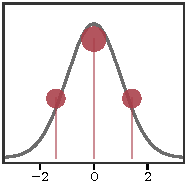
\includegraphics[width=.17\linewidth]{figures/matching-quantitative-clt/n-002.pdf} &

\includegraphics[width=.17\linewidth]{figures/matching-quantitative-clt/n-004.pdf} &
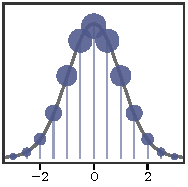
\includegraphics[width=.17\linewidth]{figures/matching-quantitative-clt/n-016.pdf} &
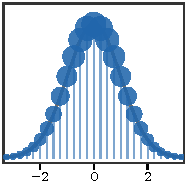
\includegraphics[width=.17\linewidth]{figures/matching-quantitative-clt/n-064.pdf}
\end{tabular}
\caption{Central-limit theorem for normalized Bernoulli sums. Starting from $\alpha_0=\frac12(\delta_{-1}+\delta_1)$, the law of $Z_n=n^{-1/2}\sum_{i=1}^n X_i$ remains discrete, but its rescaled atom heights approach the standard Gaussian density shown in gray. The Wasserstein Berry--Esseen bound below quantifies this weak convergence by a $\Wass_1$ distance.}
\label{fig:matching-quantitative-clt}
\end{figure}

\begin{prop}[Berry--Esseen bound in $\Wass_1$]\label{prop-berry-esseen-w1}
	Let $(X_i)_{i=1}^n$ be i.i.d. real random variables such that $\EE X_i=0$, $\EE X_i^2=1$ and $\EE |X_i|^3<+\infty$. If $\alpha_n$ is the law of $n^{-1/2}\sum_i X_i$ and $\gamma$ is the standard Gaussian law, then
	\[
		\Wass_1(\alpha_n,\gamma)
		\leq
		\frac{C\,\EE |X_1|^3}{\sqrt n},
	\]
	where $C$ is a universal constant.
\end{prop}

\begin{proof}
	We give the standard Stein-method sketch. By Kantorovich--Rubinstein duality,
	\[
		\Wass_1(\alpha_n,\gamma)
		=
		\sup_{\Lip(h)\leq1}
		\left|\EE h(S_n)-\EE h(G)\right|,
		\qquad
		S_n=n^{-1/2}\sum_i X_i,\ G\sim\gamma.
	\]
	For each such $h$, solve Stein's equation
	\[
		f_h'(x)-x f_h(x)=h(x)-\EE h(G).
	\]
	The solution satisfies uniform derivative bounds depending only on the Lipschitz constant of $h$. Hence
	\[
		\EE h(S_n)-\EE h(G)=\EE[f_h'(S_n)-S_nf_h(S_n)].
	\]
	Expanding $f_h'(S_n)$ and $f_h(S_n)$ by replacing the summands one at a time, the first- and second-order terms cancel because $\EE X_i=0$ and $\EE X_i^2=1$. The Taylor remainder is bounded by $C\sum_i \EE |X_i/\sqrt n|^3$, which gives the displayed $n^{-1/2}$ rate. This is the Wasserstein form of the Berry--Esseen theorem; sharper constants and higher-order transport-distance refinements are studied in~\cite{bobkov2018berry,rio2011asymptotic}.
\end{proof}


%%%%%
\paragraph{Applications and implications}

The practical value of Wasserstein distances is that they provide a geometric loss on probability measures. In barycenter problems, minimizing $\sum_s\la_s\Wass_2^2(\al,\be_s)$ produces an average distribution that respects displacement rather than pointwise density interpolation, which is crucial for shape and image averaging~\cite{Carlier_wasserstein_barycenter,CuturiBarycenter,2015-solomon-siggraph}. In registration and morphing, OT penalizes how far mass travels, so it naturally encodes spatial deformations and correspondences~\cite{haker2004optimal,peyre2012wasserstein,GramfortPC15}. In statistical fitting, one can estimate a parametric measure $\theta\mapsto\al_\theta$ from data $\be$ by minimizing $\theta\mapsto\Wass_p(\al_\theta,\be)$; this remains meaningful even when the model and empirical measure are mutually singular, unlike likelihood or $\KL$ objectives~\cite{CanasRosasco,FrognerNIPS}.
